%!TEX root = manual.tex
%===============================================================================
\chapter{Install a native programming environment}\label{ch:Assignment1}

The aim of this assignment is to install a native programming environment for the Ada language on the student PC. This environment will later be extended with cross-compilation tools for the STM32 board to be used in the laboratory. 

The programming environment to be used is GNAT Community, an open-source software development environment freely available from AdaCore, a company specialised in providing tools and solutions for developing high-integrity software,
\section{Download and install GNAT}
The GNAT Community compilation system can be downloaded from \url{https://www.adacore.com/download/more}. Installation packages for Windows, MacOS and GNU Linux are available at the download page. The file {\tt README.txt} provides installation instructions, which are summarised as follows:
\subsection{Windows}
\begin{enumerate}
\item Download the file {\tt gnat-2021-20210519-x86\_64-windows64-bin.exe}
\item Run the file and follow the instructions.
\end{enumerate}
\subsection{MacOS}
\begin{enumerate}
\item Download the file {\tt gnat-2020-20200818-x86\_64-darwin-bin.dmg}
\item Open the dmg disk and execute the application inside it. In order to circumvent the system protection, control-click on the file and then click on ``opens" in the emergent window.
\end{enumerate}
Notice that you need to have installed the Xcode application to install GNAT. If you still see the following error:
\begin{verbatim}
ld: library not found for -lSystem
\end{verbatim}
then you might have to execute the following:
\begin{verbatim}
xcode-select -s /Applications/Xcode.app/Contents/Developer
\end{verbatim}
\subsection{GNU Linux}
\begin{enumerate}
\item Download the file {\tt gnat-2021-20210519-x86\_64-linux-bin}
\item You will need to make the package executable before running it. In a command prompt, execute the following command:
\begin{verbatim}
     chmod +x path\_to\_the\_package.bin
\end{verbatim}
and execute the package. The {\tt README.txt} file contains additional installation and execution instructions.
\end{enumerate}

\section{Test the installation with a simple program}

The GNAT compilation system includes the GPS (GNAT programming studio) programming environment, which allows users to edit, compile, and run Ada and C programs. Figure\ref{fig:gps} shows the main GPS window, which is composed of the following areas:

\begin{figure}[h]
            \centering{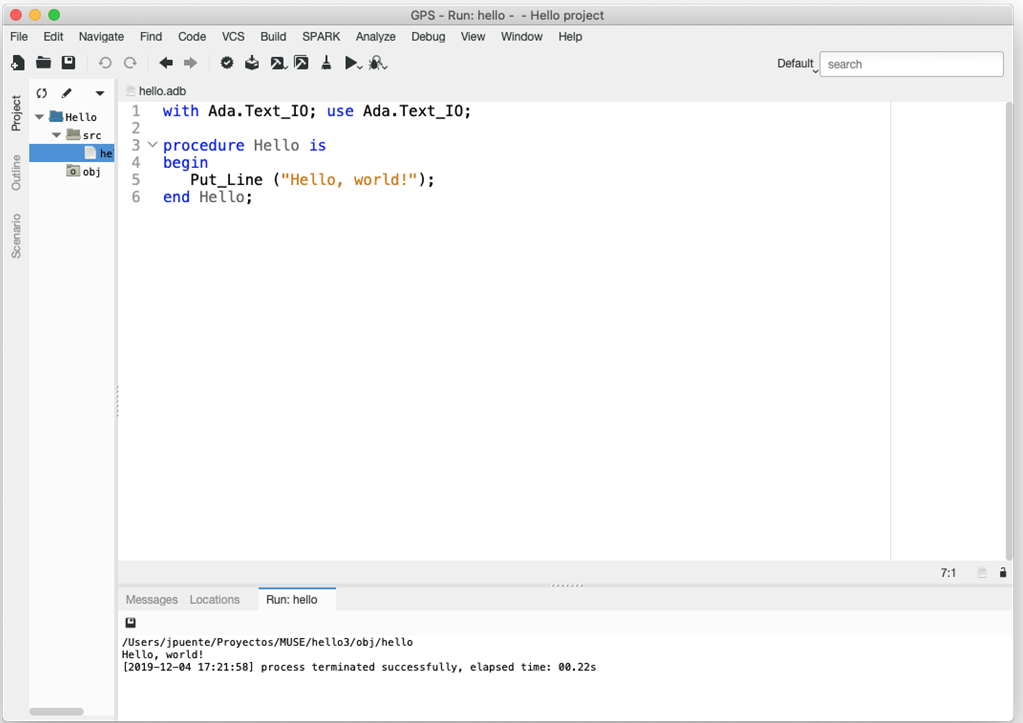
\includegraphics[width=\textwidth,keepaspectratio]{gps.png}}
            \caption{GNAT Programming Studio (GPS).}
            \label{fig:gps}
\end{figure}

\begin{itemize}
\item	a menu bar at the top
\item	a tool bar under the menu bar
\item	on the left, a notebook allowing you to switch between Project, Outline and Scenario views
\item	the working area in the center
\item	the messages window at the bottom
\end{itemize}

GPS organises source code in projects. A project is a set of source files which are compiled together in order to produce a single binary executable. 
Before starting you will need to create a folder to store your software projects. The recommendation is to create a folder named OBDH\_LABS in a directory of your choice.
The next activity is to write and run a simple Ada program using GPS:
\begin{enumerate}
\item 	Create a new project by clicking on {\tt File} $\rightarrow$ {\tt New Project} ... in the top menu. Choose the {\tt Simple Ada Project} template.
\item	Choose a folder to deploy the project, e.g. OBDH\_LABS/LAB1. Set the project name to {\tt Hello} and the main name also to {\tt Hello}.
\item	Double click on the {\tt hello.adb} file in the project view to open the file in the working area. 
\item	Edit the file in the working area so that it has the same content as in figure\ref{fig:gps}.
\item	Build and run the executable by clicking on the $\rhd$ symbol in the tool bar. You should see a number of compilation-related messages and, if everything is right, you will see the text ``Hello, world!" in the Run tab of the bottom window.
\end{enumerate}
%\begin{figure}[h]
%            \centering{\includegraphics[width=\textwidth,keepaspectratio]{gpshello.png}}
%            \caption{Hello world demo program.}
%            \label{fig:gpshello}
%\end{figure}

